\chapter{Märkte und Marktinterventionen}

\section{Märkte}
Das Konzept des Marktgleichgewichts ist ein zentrales Element der mikroökonomischen Theorie. Es beschreibt einen Zustand, in dem die angebotene Menge eines Gutes der nachgefragten Menge entspricht, sodass weder ein Angebots- noch ein Nachfrageüberschuss besteht. In der ökonomischen Analyse unterscheidet man dabei zwischen partiellem und allgemeinem Gleichgewicht. Während das allgemeine Gleichgewicht alle Märkte einer Volkswirtschaft simultan betrachtet, fokussiert sich das partielle Marktgleichgewicht auf einen einzelnen Markt unter der Annahme, dass andere Märkte unbeeinflusst bleiben.
\begin{definition}
	Gegeben seien eine Nachfragefunktion $D(p)$ und eine Angebotsfunktion $S(p)$ für ein Gut auf einem isolierten Markt.
	Ein partielles Marktgleichgewicht ist ein Preis-Mengen-Paar $(p^*,q^*)$, so dass gilt:
	\[
		D(p^*) = S(p^*) = q^*
		.\]
\end{definition}

Betrachten wir die Stabilitätsbedingung, das heißt, wenn gilt
\[
	\frac{\mathrm{d}}{\mathrm{d}p} \left( S(p) -D(p) \right) \mid_{p=p^*} > 0
	.\]
Dies führt dazu, dass ein Preisanstieg oberhalb $p^*$ zu einem Angebotsüberschuss führt.
Analog geht mit einem Preisrückgang ein Nachfrageüberschuss einher.


\begin{figure}[h]
	\caption{partielles Marktgleichgewicht, mit linearen Nachfrage- und Angebotskurve}
	\begin{center}
		\begin{tikzpicture}[scale=1.2]
			% Achsen
			\draw[->] (0,0) -- (6,0) node[right] {Menge $q$};
			\draw[->] (0,0) -- (0,5) node[above] {Preis $p$};

			% Nachfragefunktion D(p)
			\draw[thick,blue] (0.5,4.5) -- (5.5,0.5) node[below right] {$D(p)$};

			% Angebotsfunktion S(p)
			\draw[thick,red] (0.5,0.5) -- (5.5,4.5) node[above right] {$S(p)$};

			% Gleichgewichtspunkt
			\draw[dashed] (3,0) -- (3,2.5);
			\draw[dashed] (0,2.5) -- (3,2.5);
			\filldraw[black] (3,2.5) circle (2pt) node[above right] {$(q^*, p^*)$};

			% Achsenbeschriftungen
			\node at (3,-0.3) {$q^*$};
			\node at (-0.3,2.5) {$p^*$};

		\end{tikzpicture}

	\end{center}
\end{figure}

Das partielle Marktgleichgewicht kann benutzt werden um zu analysieren was passiert, wenn sich Angebot oder Nachfrage verändern.
Eine solche Analyse als komperative Statik bezeichnet.

%\begin{figure}
	\begin{center}
	%	\caption{Nachfrage und Angebotsveränderung}
		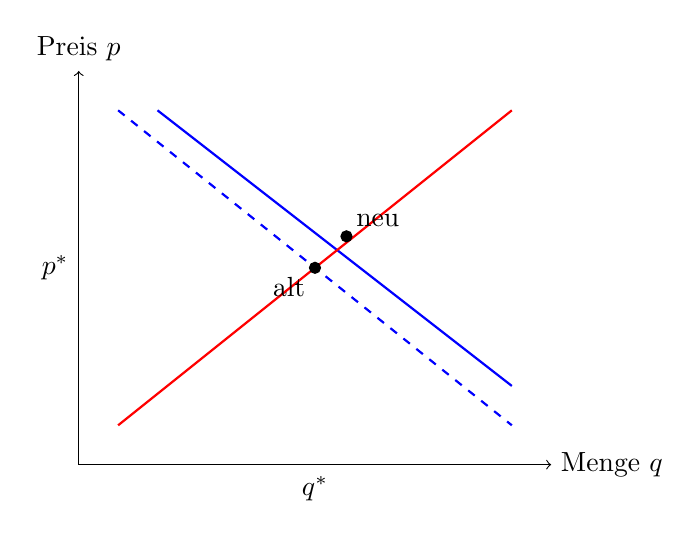
\begin{tikzpicture}[scale=1]
			% Achsen
			\draw[->] (0,0) -- (6,0) node[right] {Menge $q$};
			\draw[->] (0,0) -- (0,5) node[above] {Preis $p$};

			% Alte Nachfrage
			\draw[thick,blue,dashed] (0.5,4.5) -- (5.5,0.5);

			% Neue Nachfrage
			\draw[thick,blue] (1,4.5) -- (5.5,1);

			% Angebot
			\draw[thick,red] (0.5,0.5) -- (5.5,4.5);

			% Gleichgewichtspunkte
			\filldraw[black] (3,2.5) circle (2pt) node[below left] {alt};
			\filldraw[black] (3.4,2.9) circle (2pt) node[above right] {neu};

			% Achsenbeschriftungen
			\node at (3,-0.3) {$q^*$};
			\node at (-0.3,2.5) {$p^*$};

		\end{tikzpicture}
    \end{center}
        Ein Anstieg des Einkommens oder eine Präferenzänderung erhöht die Nachfrage, verschiebt die Kurve nach rechts und führt zu einem höheren Gleichgewichtspreis und einer größeren Gleichgewichtsmenge. 
        \begin{center}
		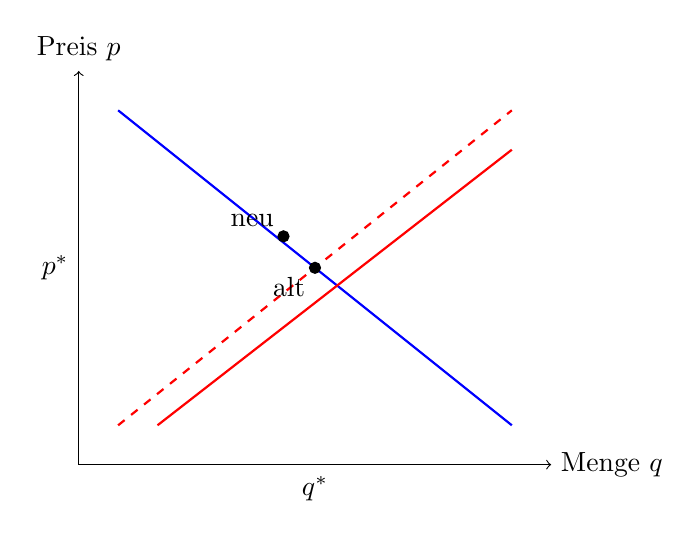
\begin{tikzpicture}[scale=1]
			% Achsen
			\draw[->] (0,0) -- (6,0) node[right] {Menge $q$};
			\draw[->] (0,0) -- (0,5) node[above] {Preis $p$};

			% Nachfrage
			\draw[thick,blue] (0.5,4.5) -- (5.5,0.5);

			% Altes Angebot
			\draw[thick,red,dashed] (0.5,0.5) -- (5.5,4.5);

			% Neues Angebot (linksverschoben)
			\draw[thick,red] (1,0.5) -- (5.5,4);

			% Gleichgewichtspunkte
			\filldraw[black] (3,2.5) circle (2pt) node[below left] {alt};
			\filldraw[black] (2.6,2.9) circle (2pt) node[above left] {neu};

			% Achsenbeschriftungen
			\node at (3,-0.3) {$q^*$};
			\node at (-0.3,2.5) {$p^*$};

		\end{tikzpicture}

	\end{center}
Sinkende Produktionskosten oder technologische Innovationen verschieben die Angebotskurve nach rechts und senken den Gleichgewichtspreis bei gleichzeitig höherer Gleichgewichtsmenge. 

%\end{figure}


\begin{remark}
    In dem wir $D(p)$ und $S(p)$ betrachten, nehmen wir implizit an, dass Konsumenten und Produzenten \emph{Preisnehmer} sind, also Preise nicht beeinflussen können.  
\end{remark}



Obwohl das partielle Marktgleichgewicht ein nützliches Instrument für die Analyse einzelner Märkte ist, besitzt es auch Einschränkungen, wie beispielsweise die Vernachlässung von Wechselwirkungen zwischen verschiedenen Märkten, die vereinfachten Annahmen und nur eine kurzfristige Betrachtung. 

\begin{example}[Feuer]
tbd
\end{example}


\section{Marktinterventionen}



In unserem bisherigem vorgehen, haben wir staatliche Eingriffe oder andere Friktionen vernachlässigt.
Typischerweise existieren diese, oft sind diese Eingriffe Steuern.

\subsection{Steuern}

Zahlen Produzenten die Steuern, dann verändert sich die Nachfragekurve der Konsumenten nicht, jedoch verändert sich die Angebotskurve bei einer Steuer $t$ gerade:
\[
S'(p) = S(p-t)
,\]
damit verschiebt sich diese genau um $t$ nach oben. 
Zahlen nun Konsumenten die Steuer ergibt sich analog:
\[
D'(p) = D(p+t)
,\]
damit verschiebt nicht die Nachfragekurve genau um $t$ nach unten.

\begin{figure}[h!]
\centering
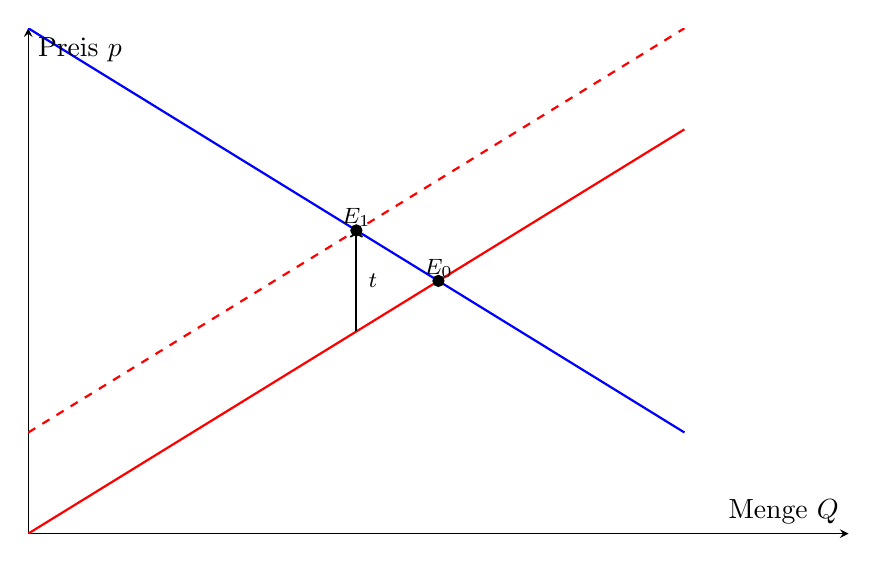
\begin{tikzpicture}
\begin{axis}[
    axis lines = middle,
    xlabel = {Menge \( Q \)},
    ylabel = {Preis \( p \)},
    xtick = \empty,
    ytick = \empty,
    ymin=0, ymax=20,
    xmin=0, xmax=20,
    width=12cm, height=8cm
]

% Nachfragekurve
\addplot[
    domain=0:16,
    samples=100,
    color=blue,
    thick
]
{20 - x};

% Angebotskurve ohne Steuer
\addplot[
    domain=0:16,
    samples=100,
    color=red,
    thick
]
{x};

% Angebotskurve mit Steuer
\addplot[
    domain=0:16,
    samples=100,
    color=red,
    dashed,
    thick
]
{x + 4};

% Gleichgewicht ohne Steuer
\addplot[only marks, mark=*] coordinates {(10,10)};
\node at (axis cs:10,10.5) {\footnotesize \( E_0 \)};

% Gleichgewicht mit Steuer
\addplot[only marks, mark=*] coordinates {(8,12)};
\node at (axis cs:8,12.5) {\footnotesize \( E_1 \)};

% Steuerbetrag
\draw [->, thick] (axis cs:8,8) -- (axis cs:8,12);
\node at (axis cs:8.4,10) {\footnotesize \( t \)};

\end{axis}
\end{tikzpicture}
\caption{Wirkung einer Mengensteuer im Marktmodell}
\end{figure}

Es entseht unabhängig davon, wer besteuert wird das gleiche Gleichgewicht, wenn die Steuer gleich ist. Jedoch entsteht je nach Besteuerung ein Wohlfahrtsverlust, für entweder Konsument oder Produzent, denn ein Teil der Einnahmen wird nun an den Staat abgegeben.
\begin{definition}
    Die \defemph{Gesamtwohlfahrt} ergibt sich aus der Summe von Konsumenten-, Produzentenrente und staatliche Einnahmen:
    \[
        \operatorname{TW} = \operatorname{CS} + \operatorname{PS} + \operatorname{GR}
    .\] 
    Der Wohlfahrtsverlust ergibt sich aus dem Wert, den die Gesamtwohlfahrt nach der Steuer sinkt. 
\end{definition}

\subsection{Preisgrenzen}

Ein Höchstpreis ist ein gesetzlich festgelegter Maximalpreis \( p_{\text{max}} \), der unterhalb des Gleichgewichtspreises liegt. Er führt zu einem Nachfrageüberhang.

\begin{figure}[h!]
\centering
\begin{tikzpicture}
\begin{axis}[
    axis lines = middle,
    xlabel = {Menge \( Q \)},
    ylabel = {Preis \( p \)},
    xtick = \empty,
    ytick = \empty,
    ymin=0, ymax=20,
    xmin=0, xmax=20,
    width=12cm, height=8cm
]

% Nachfragekurve
\addplot[
    domain=0:16, 
    samples=100, 
    color=blue, 
    thick
]
{20 - x};

% Angebotskurve
\addplot[
    domain=0:16, 
    samples=100, 
    color=red, 
    thick
]
{x};

% Gleichgewicht
\addplot[only marks, mark=*] coordinates {(10,10)};
\node at (axis cs:10,10.5) {\footnotesize \( E \)};

% Höchstpreislinie
\addplot[domain=0:20, samples=2, dashed, thick] {6};
\node at (axis cs:1,6.5) {\footnotesize \( p_{\text{max}} \)};

\end{axis}
\end{tikzpicture}
\caption{Wirkung einer Preisobergrenze}
\end{figure}

Ein Mindestpreis \( p_{\text{min}} \) liegt oberhalb des Gleichgewichtspreises und führt zu einem Angebotsüberschuss.



\subsection{Zölle und Quoten}

Im Kontext des partiellen Marktgleichgewichts lässt sich auch der Außenhandel eines Landes modellieren. Wird der Inlandsmarkt für Importe geöffnet, passt sich der inländische Preis an das niedrigere Weltmarktniveau an. Der Staat kann mittels **Zöllen** und **Importquoten** eingreifen, um die heimische Produktion zu schützen. Diese Maßnahmen verändern Preis, Menge und Wohlfahrt.


Damit wir Zöllen und Quoten überhaupt behandeln können, müssen wir handel zu lassen.


\begin{definition} \index{Freihandel}
	Eine Situation, in der uneingeschränkt gehandelt werden kann, wird als
	\defemph{Freihandel} bezeichnet.
\end{definition}

Handel ergibt nur Sinn, wenn der internationale Angebotspreis unterhalb des lokalen Angebotspreis ist.

\begin{definition}
    Ein \defemph{Zoll} ist ein Preisaufschlag auf importierte Güter. 
\end{definition}
Im Modell bewirkt ein Zoll, dass der Inlandspreis für Importe über den Weltmarktpreis steigt. Dies führt zu einer Erhöhung der inländischen Produktion, einer Reduktion der Importe und einem höheren Verbraucherpreis.

\begin{figure}[h!]
\centering
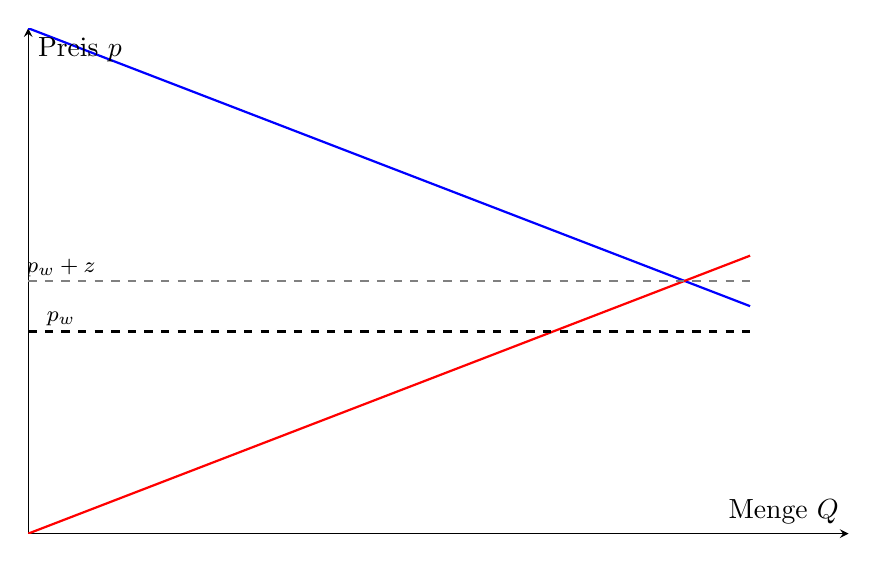
\begin{tikzpicture}
\begin{axis}[
    axis lines = middle,
    xlabel = {Menge \( Q \)},
    ylabel = {Preis \( p \)},
    xtick = \empty,
    ytick = \empty,
    ymin=0, ymax=20,
    xmin=0, xmax=25,
    width=12cm, height=8cm
]

% Nachfragekurve
\addplot[
    domain=0:22,
    samples=100,
    color=blue,
    thick
]
{20 - 0.5*x};

% Angebotskurve
\addplot[
    domain=0:22,
    samples=100,
    color=red,
    thick
]
{0.5*x};

% Weltmarktpreis ohne Zoll
\addplot[domain=0:22, samples=2, dashed, thick] {8};
\node at (axis cs:1,8.5) {\footnotesize \( p_w \)};

% Weltmarktpreis mit Zoll
\addplot[domain=0:22, samples=2, dashed, thick, color=gray] {10};
\node at (axis cs:1,10.5) {\footnotesize \( p_w + z \)};

\end{axis}
\end{tikzpicture}
\caption{Wirkung eines Importzolls im Marktmodell}
\end{figure}


Neben Zoll auf die Güter, kann es auch Quoten geben, die den Import auf gewisse Güter auf eine Menge beschränkt wird.
\begin{definition}
    Eine \defemph{Importquote} begrenzt die maximal zulässige Importmenge eines Gutes. 
\end{definition}
 Sie wirkt ähnlich wie ein Zoll, jedoch ohne staatliches Einnahmepotenzial, da die Importbeschränkung typischerweise über Lizenzen oder Kontingente verteilt wird.



\section{Allgemeines Gleichgewicht}
Im partiellen Gleichgewichtsmodell haben wir nur ein einziges Gut
angeschaut und gefragt für welchen Preis \enquote{Angebot gleich Nachfrage} gilt.

Allgemein versuchen wir, die Variablen, die im partiellen Gleichgewichtsmodell exogen gegeben sind,
zu endogenisieren.


\begin{definition}[Allgemeines Marktgleichgewicht]
Ein Preis-Allokations-Paar \( (p^*, (x_1^*, \dots, x_I^*)) \) heißt \emph{allgemeines Marktgleichgewicht}, wenn
\begin{itemize}
    \item für alle \( i \) gilt: \( x_i^* \) löst
    \[
    \max_{x_i \in \mathbb{R}^L_+} u_i(x_i) \quad \text{s.t.} \quad p^* \cdot x_i \leq p^* \cdot \omega_i
    \]
    \item und für alle Güter \( \ell = 1, \dots, L \) gilt:
    \[
    \sum_{i=1}^I x_{i\ell}^* \leq \sum_{i=1}^I \omega_{i\ell}
    \]
    mit Gleichheit, falls \( p^*_\ell > 0 \)
\end{itemize}
\end{definition}

\subsection{Walras'sches Gesetz}

\begin{proposition}[Walras’sches Gesetz]
Für jede Preis-Nachfrage-Kombination gilt:
\[
p \cdot \left( \sum_{i=1}^I x_i(p) - \omega_i \right) = 0
\]
\end{proposition}

\begin{proof}
Da jeder Konsument im Gleichgewicht sein Budget vollständig ausnutzt, gilt:
\[
p \cdot x_i(p) = p \cdot \omega_i
\]
für alle \( i \).  
Summieren über alle Konsumenten ergibt:
\[
p \cdot \left( \sum_{i=1}^I x_i(p) - \omega_i \right) = \sum_{i=1}^I \left(p \cdot x_i(p) - p \cdot \omega_i\right) = 0
\]
\end{proof}
Wenn auf allen Märkten Preise herrschen und Konsumenten ihr gesamtes Einkommen ausgeben, dann kann die Überschussnachfrage in einem Markt nicht positiv sein, ohne dass sie in einem anderen Markt negativ ist.

\begin{remark}
Wenn $L-1$ Märkte im Gleichgewicht sind, so ist der $L$-te Markt automatisch auch im Gleichgewicht.  
\end{remark}

\begin{example}
Wenn es zwei Güter gibt und ein Überschussnachfrage von 10 Einheiten für Gut 1 besteht, dann muss ein Überschussangebot von entsprechendem Wert in Gut 2 existieren, um die Wertbilanz auszugleichen.
\end{example}
\subsection{Fundamentalsatz der Wohlfahrtsökonomik}

\begin{theorem}[Erster Wohlfahrtssatz]
Jedes allgemeine Marktgleichgewicht ist Pareto-effizient.
\end{theorem}

\begin{proof}[Beweisskizze]
Sei \( (p^*, x^*) \) ein Marktgleichgewicht.

Angenommen, es existiere eine zulässige Allokation \( (\tilde{x}_1, \dots, \tilde{x}_I) \) mit
\begin{itemize}
    \item \( \sum_{i=1}^I \tilde{x}_i \leq \sum_{i=1}^I \omega_i \)
    \item \( u_i(\tilde{x}_i) \geq u_i(x_i^*) \) für alle \( i \)
    \item und \( u_j(\tilde{x}_j) > u_j(x_j^*) \) für mindestens ein \( j \)
\end{itemize}

Da jeder Konsument sein Nutzenmaximum im Budgetbereich erreicht, muss jede Verbesserung des Nutzens mit höheren Ausgaben verbunden sein:
\[
p^* \cdot \tilde{x}_i \geq p^* \cdot \omega_i
\]
für alle \( i \), wobei striktes Ungleichgewicht für mindestens ein \( j \) gelten muss.

Summieren liefert:
\[
p^* \cdot \left( \sum_{i=1}^I \tilde{x}_i \right) > p^* \cdot \left( \sum_{i=1}^I \omega_i \right)
\]

Da aber per Annahme \( \sum_i \tilde{x}_i \leq \sum_i \omega_i \) und \( p^* \gg 0 \), ergibt sich ein Widerspruch.

Folglich existiert keine solche Allokation.  
Damit ist \( x^* \) Pareto-effizient.
\end{proof}

Der freie Markt führt unter bestimmten Bedingungen (keine Externalitäten, vollständige Konkurrenz, vollständige Märkte) zu einer Allokation der Ressourcen, bei der niemand besser gestellt werden kann, ohne jemand anderen schlechter zu stellen.


\begin{remark}
Der Satz sagt nichts darüber aus, wie „gerecht“ das Ergebnis ist — nur, dass es effizient ist.
\end{remark}

\begin{fluff}[Intuition]
    Weil jeder Konsument sein Budget maximiert und Güter vollständig gehandelt werden. Eine Verbesserung für einen Konsumenten würde zusätzliche Ressourcen beanspruchen, die anderen Konsumenten entzogen werden müssten — was im Gleichgewicht nicht möglich ist.
\end{fluff}



\begin{theorem}[zweiter Fundamentalsatz]
ede Pareto-effiziente Allokation kann durch geeignete Umverteilung der Anfangsausstattungen als kompetitives Gleichgewicht realisiert werden.
\end{theorem}


\section{Kapitaleinkommen \& Besteuerung}
Einkommen aus Kapital fließt vor allem reichen Leuten zu. Viele Leute
empfinden deshalb eine Kapitalsteuer, die mindestens so hoch ist wie eine
Lohnsteuer, als gerecht. Parteien wie z.B. die FDP argumentieren dagegen
manchmal, dass eine geringe Kapitalsteuer allen Gesellschaftsschichten zu
Gute kommt, da ein günstiges Investitionsklima den Arbeitsmarkt
stimuliert, Gehälter erhöht und Arbeitslosigkeit senkt.
Ist es der Fall, dass eine geringere Kapitalsteuer zu höheren Gehältern für
Arbeiter führt?

\begin{remark}
	Ein weiteres Argument gegen hohe Steuern auf Kapital ist
	Steuerflucht, getreu dem Motto \enquote{Besser $25$ Prozent von X als $45$ Prozent
		von nix.}
\end{remark}


Da es aber offensichtlich ist, warum Steuerflucht als ein Argument gegen
hohe Steuern auf Kapital bzw. Kapitalerträge benutzt werden kann (und
nur die Größe des Effekts umstritten ist) werden wir uns mit der Frage
beschäftigen ob Steuern auf Kapital zu höheren Gehältern führen oder
nicht, die viel umstrittener und daher interessanter ist.


\begin{remark}
	Ist die Rendite bei Kapitalanlagen fix macht es keinen
	großen Unterschied ob Sie Kapitalerträge oder Kapitalanlagen besteuern.
\end{remark}
\begin{example}
	Nehmen wir z.B. eine Steuer auf Kapitalerträge von $25\%$. Ist die Rendite
	$10\%$ so bedeutet dies, dass von einer Kapitalanlage von $X$ Euro eine Steuer
	in der Höhe von $25\%\cdot (10\%\cdot X)$ gezahlt wird. Da $25\%\cdot (10\%\cdot X) = 2,5\%\cdot X$
	ist dies das Gleiche wie eine Steuer auf Kapitalanlagen von $2,5\%$.
	Nehmen wir einfachheitshalber an, dass Renditen für verschiedene Einlagen
	in etwa gleich sind, so macht es daher keinen Unterschied ob wir eine
	Erhöhung einer Steuer auf Kapitalanlagen oder die Erhöhung einer Steuer
	auf Kapitalerträge betrachten.
\end{example}





In intertemporalen Modellen ist das \emph{Kapitaleinkommen} das Einkommen, das Individuen aus Ersparnissen bzw. Kapitalanlagen beziehen. Die Besteuerung von Kapitaleinkommen hat wesentliche Auswirkungen auf Sparanreize, Investitionen und Konsumverhalten.

\subsection{Intertemporales Konsummodell}

Betrachtet wird ein Konsument mit Anfangseinkommen \( y_1 \) in Periode 1 und Einkommen \( y_2 \) in Periode 2. Der Konsument maximiert seinen Nutzen über den Konsum \( (c_1, c_2) \) in beiden Perioden:
\[
\max_{c_1, c_2} \; u(c_1) + \beta u(c_2)
\]
unter der intertemporalen Budgetrestriktion:
\[
c_1 + \frac{c_2}{1+r} \leq y_1 + \frac{y_2}{1+r}
\]
wobei \( r \) der Realzins ist und \( \beta \) der subjektive Diskontfaktor.

\subsection{Besteuerung von Kapitaleinkommen}

Es existieren verschiedene Steuerformen, die Kapitaleinkommen direkt oder indirekt beeinflussen:

\begin{itemize}
    \item \textbf{Zinsbesteuerung:} Ein Steuersatz \( t \) reduziert den Nettozins auf \( r(1-t) \)
    \item \textbf{Konsumsteuern:} Verursachen eine höhere relative Belastung des Konsums in der Zukunft
    \item \textbf{Kapitalertragssteuer:} Besteuert den Ertrag auf Vermögensanlagen
\end{itemize}

Die intertemporale Budgetgerade verändert sich unter Zinsbesteuerung zu:
\[
c_1 + \frac{c_2}{1+r(1-t)} \leq y_1 + \frac{y_2}{1+r(1-t)}
\]


Ein sinkender Zinsertrag mindert das Gesamteinkommen und kann je nach Präferenzstruktur sowohl zu einer Erhöhung als auch zu einer Senkung des Konsums führen.

\subsection{Optimalbesteuerungstheorie}

Die Theorie der Optimalbesteuerung beschäftigt sich mit der Frage, wie Kapitaleinkommen besteuert werden sollten, um Effizienzverluste zu minimieren und Verteilungsziele zu erreichen.

\begin{itemize}
    \item \textbf{Atkinson-Stiglitz-Theorem:} Unter bestimmten Bedingungen (homothetische Präferenzen und keine Marktunvollkommenheiten) ist es effizient, nur Konsum und nicht Kapitaleinkommen zu besteuern.
    \item \textbf{Chamley-Judd-Resultat:} In einem unendlichen Zeithorizont-Modell sollte der langfristige Steuersatz auf Kapitaleinkommen gegen null tendieren, um Kapitalakkumulation nicht zu verzerren.
\end{itemize}

\begin{remark}
In der Realität werden Kapitaleinkommen meist niedriger besteuert als Arbeitseinkommen, um Investitionsanreize zu wahren und Kapitalflucht zu vermeiden. Dies führt allerdings zu Verteilungsfragen, da Kapitaleinkommen ungleich verteilt ist.
\end{remark}

